\chapter{Introdução}
\label{cap:introducao}

O desenvolvimento tradicional de software tem se mostrado incapaz de lidar de modo eficiente com a evolução constante que os artefatos de software estão sujeitos durante seu ciclo de vida \citep{Kleppe:2003}. Os artefatos produzidos nas fases iniciais de desenvolvimento, como documento de requisitos e digramas UML, tem seu conteúdo cada vez mais distanciado do estado atual do software à medida que avançam as etapas de codificação e testes. Durante a etapa de manutenções, essa distância torna sem valor os documentos textuais e diagramas inicialmente produzidos.
A manutenção sem documentação acaba sendo feita totalmente via inspeção de código, o que torna o processo bastante improdutivo. Da mesma forma, a atualização constante dos documentos e diagramas torna o processo de desenvolvimento menos produtivo \citep{Kleppe:2003}. Além dos problemas com manutenção e produtividade, existem graves problemas acerca da interoperabilidade e dependência de plataforma, dado à vasta gama de novas tecnologias e plataformas de software que surgem cada vez mais rapidamente.
A abordagem de desenvolvimento orientada a modelos é uma resposta da academia a essa série de problemas que se apresenta ao mercado como uma alternativa ao desenvolvimento tradicional e seus artefatos \citep{Frankel:2002}. MDA (Model Driven Architecture) é um framework de desenvolvimento de software, definido pela OMG (Object Management Group), que propõe a modelagem como atividade central na construção de software.
 	A atividade de modelagem começa com a elaboração de um modelo independente de computação (CIM), que após a fase de análise origina um modelo independente de plataforma (PIM). A fase de projeto, levando em consideração a tecnologia de implementação, utiliza o PIM para gerar um modelo específico de plataforma (PSM) que nas fases seguintes é transformado em código. A cada fase os modelos se tronam menos abstratos e mais relacionados com a tecnologia adotada. 
	A definição de MDA prevê que transformações entre os níveis de modelos, ou mesmo reestruturações em um dado nível, ocorram de forma automática preservando sempre a conformidade entre os vários modelos. Nessa abordagem, desenvolvedores focariam seus esforços na criação de modelos PIM que melhor suportassem as regras de negócio do sistema e através do uso de ferramentas de transformação seriam gerados, na seqüência, modelos PSM e código fonte.
	Todo o esforço dos desenvolvedores concentrado na definição de um modelo PIM, gera ganho de produtividade e qualidade no sistema final, já que a complexidade da geração do PSM (e código fonte) torna-se responsabilidade das ferramentas de transformação. Um único PIM pode gerar PSMs para diferentes plataformas, aumentando assim a portabilidade do sistema. A manutenção, nessa abordagem, também é bastante favorecida, pois o PIM assume o papel de documentação de alto-nível do sistema e está sempre de acordo com o estado atual do mesmo, favorecendo a incorporação de novos requisitos através de mudanças no PIM seguidas de gerações automáticas de PSM e código \citep{Frankel:2002}.
	Um tipo de transformação, previsto no framework MDA, é destinado a reestruturar o modelo mantendo-o no mesmo nível. Reestruturação (refactoring) é definida em como sendo uma transformação de uma abstração em outra, de mesmo nível, preservando o comportamento externo do sistema (funcionalmente e semanticamente). A aplicação de refactorings tem como objetivo aumentar a qualidade do software através da inserção ou melhoria de requisitos não funcionais ou soft-goals (como, por exemplo, modularidade, manutenabilidade, reusabilidade). A pouca disponibilidade de ferramentas que automatizem as transformações, peça central do framework MDA, é um entrave a sua utilização plena no mercado \citep{Frankel:2002}. 


\begin{figure}[htp]
\centering
  \caption[]{\ac{lts} Estados, transições e eventos}
  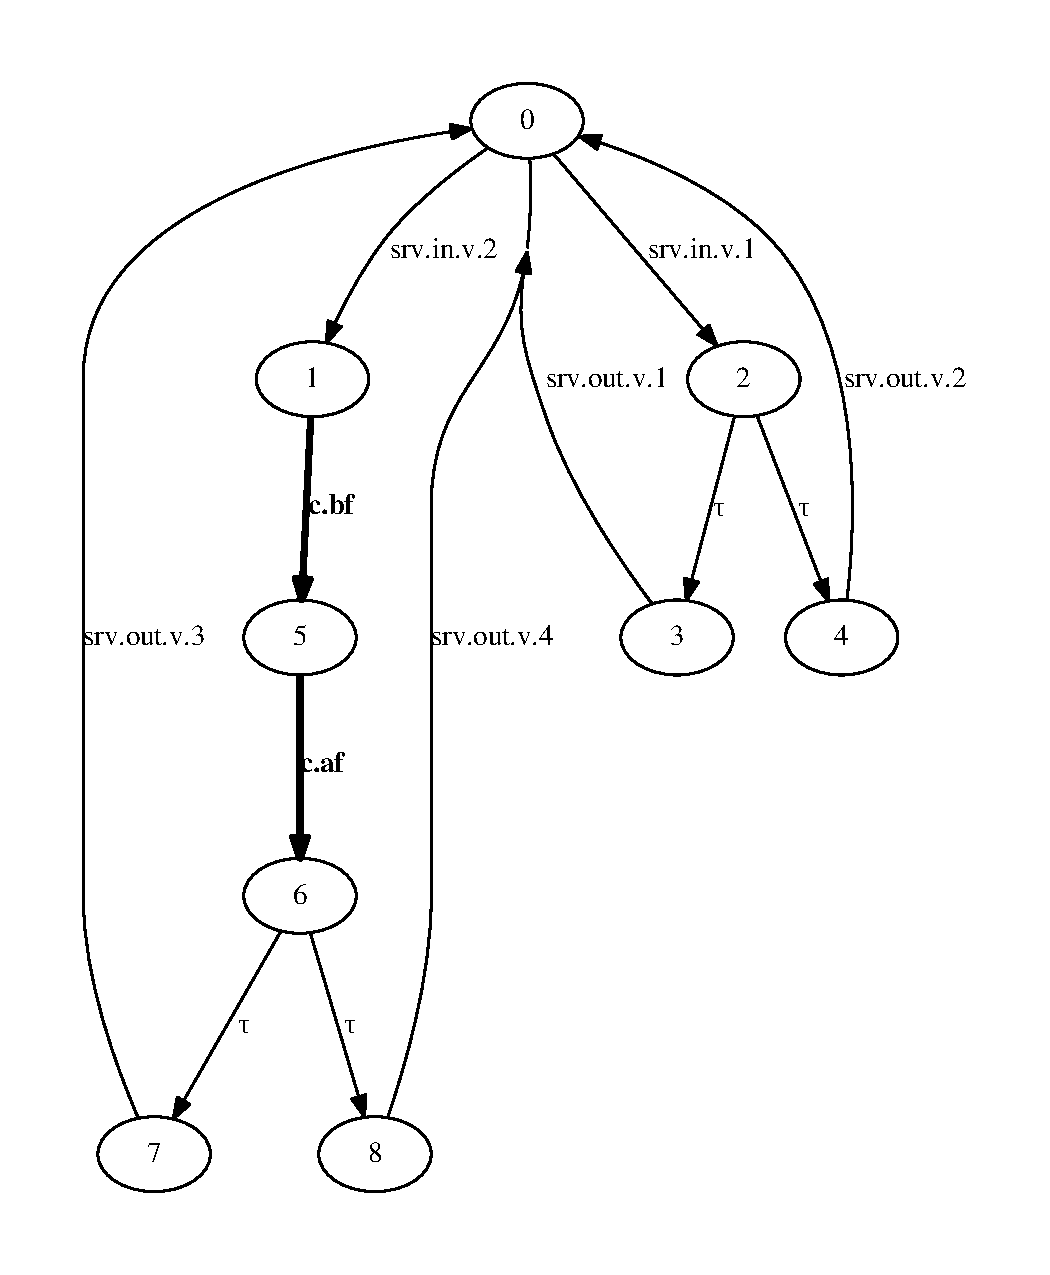
\includegraphics[width=\columnwidth]{imagens/P1andSRV-eps-converted-to.pdf}
  \footnotesize{Fonte: próprio autor}
  \label{fig:minha-imagem1}
\end{figure}

Isso é demostrado na \figref{fig:minha-imagem1}, onde...

Observe a \tabref{tbl:historico_revisoes}, é possível ver...

A equação matemática...

\begin{equation}
Z=\min E \int_{0}^{\infty} \exp(-\rho t)\left\{ \alpha^2[r(t)-x(t)]^2+
  \left[\lambda ^ {-1}\frac{\dd{x(t)}}{\dd{t}}\right]^2 \right\} \dd{t}
\end{equation}

 \section{Suporte}
Para terminar seu TCC é preciso:

\begin{enumerate}
  \item Estudar.
  \item Estudar mais.
  \item Dormir para estudar
  \item Estudar
  \item Voltar ao passo 1.
\end{enumerate}

\section{Proposta}
\lipsum[2-2]



\section{Organização deste trabalho}

\lipsum[2-2]
